\documentclass[]{report}
\renewcommand\thesection{\arabic{section}}%for page numbering in arabics
\usepackage{graphicx,tabularx}%for figures and tables
\usepackage[utf8]{inputenc} %allows special characters such as ä, ö, ỳ
\usepackage[english]{babel}  %set the language to English
\usepackage[margin=1.5in]{geometry} %change page margins 
\usepackage{sectsty}%section headers
\usepackage{algpseudocode}
\usepackage{float}
\allsectionsfont{\sffamily\large}
\subsectionfont{\sffamily\normalsize}
\linespread{1.2}% line distance
\usepackage{lipsum}% http://ctan.org/pkg/lipsum
\usepackage{caption}%use for captions on tables
%use this exact command. The style and bibliographystyle has to be authoryear (Havard). The sorting is nyt: name, year, title so that the bibliography is sorted alphabetically. firstinits=true shortens the names: Albert Einstein -> A. Einstein
\usepackage[backend=bibtex,style=authoryear,bibstyle=authoryear,sorting=nyt,firstinits=true]{biblatex}
\setlength\parindent{0pt}%include this so that your paragraphs don't indent automatically
\addbibresource{report.bib} %this attaches your bib-file, your bibliography (must be in the same folder)
\usepackage[compact]{titlesec}%include title formatting package
\setcounter{secnumdepth}{5}

% Title Page
\title{Relationship between Time Complexity and Number of Elements, within different Sorting Algorithms.}
\author{Mino Karadzhov and Kestutis Dikinis}
\date{December 10th 2021 \\Module: SEAR \\Venlo, Limburg, Netherlands}


\begin{document}

\maketitle

\begin{abstract}
This is the abstract. We are going to write this one at the end.

\pagenumbering{roman}

\end{abstract}

\tableofcontents
\setcounter{page}{3}
\listoffigures %UNCOMMENT IF YOU HAVE FIGURES
%\listoftables %UNCOMMENT IF YOU HAVE TABLES
\pagebreak

\pagenumbering{arabic}	
	
\section{Introduction}
TODO: Write about the purpose of this section, when you finish writing it.
  
\subsection{Context and Background}
	In computer science, a sorting algorithm is an algorithm that takes elements of a list and puts them into an order - ascending or descending. The most popular values used are numerical and lexicographical order. It is important to have efficient sorting for optimising other algorithms, such as merge and search algorithms, as they require data to be in sorted list.
	Whenever there is a problem to be solved, there is many ways to approach it. Even though all those approaches end up with the same result, the time it takes for each approach can be vastly different. And the best example of that is sorting algorithms.  
		- History of Algorithms.
		
		\subsection{Modern Usage, developments}
		
		Sorting algorithms are everywhere in day-to-day life in digital world. Everywhere starting from file browser in a computer - you can sort files on any parameters. Galleries in mobile phones - images sorted by date, contacts sorted alphabetically . Searching for a product in online store will have an option to sort products in many ways. 
		Commercial computing: government organisations, financial institutions, and commercial enterprises organise much of this information by sorting it. Whether the information is accounts to be sorted by name or number, transactions to be sorted by time or place, mail to be sorted by postal code or address, files to be sorted by name or date, or whatever, processing such data is sure to involve a sorting algorithm somewhere along the way. 
		Numerical computations: Scientific computing is often concerned with accuracy (how close are we to the true answer?). Accuracy is extremely important when we are performing millions of computations with estimated values such as the floating-point representation of real numbers that we commonly use on computers. Some numerical algorithms use priority queues and sorting to control accuracy in calculations.All in all, all any and every kind of list there is has been sorted in some way or another, as it is hard for a human to make use of unsorted data.[2]
		
\subsection{Sorting algorithm explanations}
		Bubblesort is a simple sorting algorithm that belongs to the family of comparison sorting. It works by repeatedly stepping through the list to be sorted, comparing two items at a time and swapping them if they are in the wrong order. Bubblesort has a worst-case complexity O(n 2 ) and in the best case O(n). Its memory complexity is O(1). [2]

		Heapsort is a comparison-based sorting algorithm, and is part of the Selection sort family. Although somewhat slower in practice on most machines than a good implementation of Quicksort, it has the advantage of a worst-case O(n log n) runtime.[2]

		Mergesort belongs to the family of comparison-based sorting. It has an average and worst-case performance of O(n log n). Unfortunately, Mergesort requires three times the memory of in-place algorithms such as Insertionsort. [2]

		Selection sort belongs to the family of in-place comparison sorting. It typically searches for the minimum value, exchanges it with the value in the first position and repeats the first two steps for the remaining list. On average Selection sort has a O(n 2 ) complexity that makes it inefficient on large lists. Selection sort typically outperforms Bubblesort but is generally outperformed by Insertionsort.[2]

		On the other side of the sorting algorithm spectrum there is BogoSort. It was designed as a joke about how not to design sorting algorithms. BogoSort takes and randomly swaps places all elements of the list and repeats it until the list is sorted. Complexity of BogoSort algorithm is O((n+1)!).

\subsection{Hypothesis, Problems and Considerations}
		- Our Hypothesis that we are going to see a linear growth of the Time Complexity, towards Size of Collection.
		- What is Time Complexity ?
		- Why is Time Complexity important? 
		-  What could affect the Time Complexity.
		- External factors that can affect the Time Complexity.
		\subsubsection{Time Complexity and the importance of it.}
		\subsubsection{Factors, operating on Time Complexity.}
		\subsubsection{Different methods of approaching our Research question.}
		
\section{Methodology}
In order to approve or deny our initial hypothesis, an Empirical Analysis of certain  Sorting Algorithms was conducted. This chapter of the paper describes the process of conducting the experiment and creating the proper experimental environment. The subject group of Sorting Algorithms includes: QuickSort, BubbleSort, SelectionSort and HeapSort. The main goal of the analysis is to observe changes of the Time  Complexity, when the same algorithm is given the task to sort a collection of a certain size. Each observation of our experiment includes a task of sorting, performed by one of the sorting algorithms from our subject group, performed on a collection of certain size.\\
In order to conduct the Empirical Analysis, a custom-made Java application was developed and used in the process. The main purpose  of which is to create a proper experimental environment , that is going to allow close observation of each algorithm from our subject group. \\
The overall goal is to gain an output, which allows data analysis on the covariation between the Size of Collection, used for the observation, and the time that was required for the algorithm to fully perform the sorting task.
	\subsection{Working Implementation of our Algorithms.}
	One requirement of the Empirical Analysis is a working implementation of the Sorting Algorithms, that are going to be used for the experiment. Due to this, the Java programming language was used to create working implementations of each one of the four members of our Subject group. All of the concrete implementations of the Algorithms implement a common interface, towards which the testing is being conducted.
	\subsection{Developing and using our experimental environment.}
	In order to serve the need of a proper experimental environment  for conducting the Analysis, Petko was developed. Petko is the name of the custom-made  Algorithm Analysis tool, that generates unsorted collections of a fixed size and uses sorters(Sorting Algorithms) to conduct the sorting operation. The latter is being closely monitored and the time required for each sorting is being recorded in an output file, in a format of nanoseconds. \\
	Each Algorithm is used to perform 18 different observations. Each Observation requires the algorithm to sort an unsorted collection of a fixed size. The size of the unordered collection grows with each following observation. The first observation of each algorithm starts with performing a sorting on a Collection with a number of elements of 2, whereas the last(18th) observation provides the Algorithm with an unsorted collection of 262144 elements. The growth of Collection Size is Logarithmic with base 2. Respectively, this means that the first collection for sorting is with size 2$^{1}$, whereas the collection for the last observation has a size equal to 2$^{18}$. \\
	Petko actively uses the Java.time integrated library, in order to measure the Duration of time between the start and end of the sorting process. That is made possible, by placing an Instant at the Start and End point of each Algorithm execution. The following PseudoCode provides a brief description of the technique:
	\begin{algorithmic}[H]
		\State $startPoint \gets Instant.now()$
		\State $sort()$
		\State $endPoint \gets Instant.now()$
		\State $timeComplexity \gets Duration.between(startPoint, endPoint)$
		\end{algorithmic} 
		 Each Observation records the Sorting Algorithm that is being used, the TimeComplexity of the observation and the Size of Collection. This output is being gathered and recored into an external File under the .csv extension. 
		\subsection{Data Analysis and Visualisation}
		Petko's output file provides a great base for conducting Data Analysis on the results of the observations. By doing this, it is possible to identify and study certain patterns in the covariation between Time Complexity and Size of Collection. The same output file was imported into R and the findings were visualised, thanks to the tidyverse library.
		\section{Results}
	This section provides a detailed overview of the experimental results.
\subsection{Experimental Results}
After conducting the Emperical Analysis, 72 datapoints were generated. The same visualised on a ScatterPlot have the following view:

\begin{figure}
	\centering
	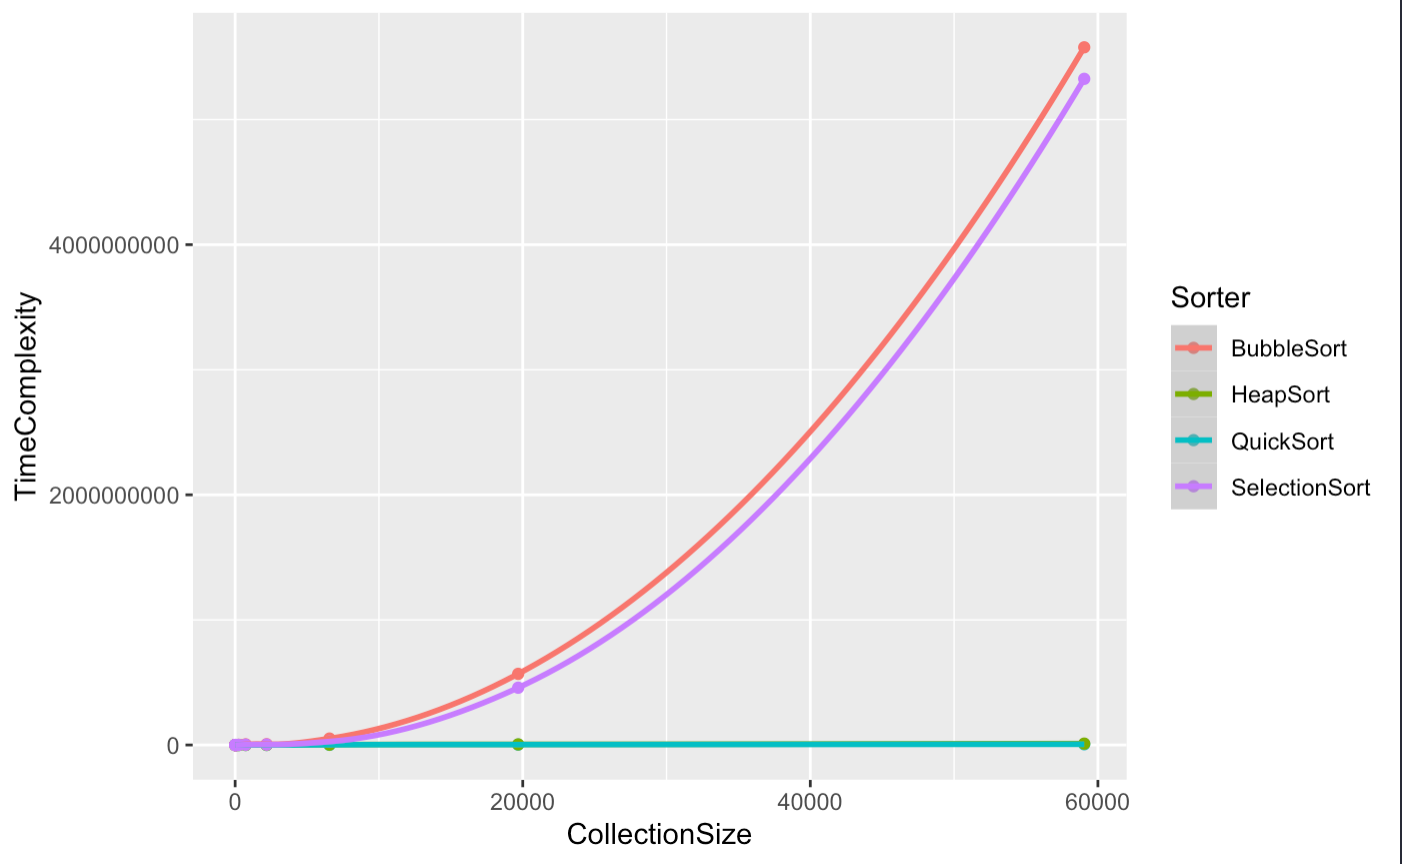
\includegraphics[width=0.7\linewidth]{ResultsOverallView}
	\caption[Figure 3.1:]{Overall view of the Experimental results.}
	\label{fig:resultsoverallview}
\end{figure}
\newpage
As we can clearly see from the above diagram, the relationship between Time Complexity and Collection Size differes between each one of the Sorters. In addition to this, we can easily identify a sharp growth of BubbleSort and SelectionSort time complexities, when the Collection size becomes more than 20 000 elements. On the other hand, looking at the QuickSort and HeapSort, we can easily observe a relationship, which can be described as similliar to Constant Time Complexity.
Taking the above into account, we can easily identify 2 sub-groups of sorters - One, where  TimeComplexity appears to be constant and One, where we can clearly see a Time Complexity growth, similliar to a Linear Growth.\\
Since the two sub-groups are vastly contrasting on the Overall view, this may be a reason why we are missing certain patterns on our visualisation.

\begin{figure}
	\centering
	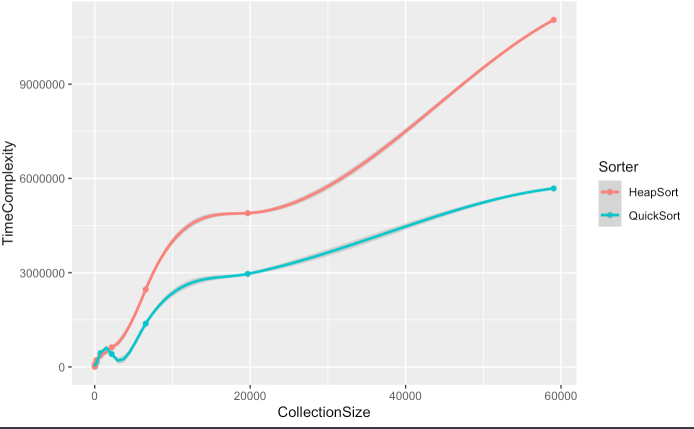
\includegraphics[width=0.7\linewidth]{OverviewOfConstantTimeComplexityAlgorithms}
	\caption[Figure 3.2]{Focused view on the sub-group with lower time complexity.}
	\label{fig:overviewofconstanttimecomplexityalgorithms}
\end{figure}
\newpage	
After creating a separate visualisation for the sub-group with lower Time Complexity, we can see more regarding the growth of Time Complexity, as the overlapping on the overal view did not provide a high level of detail. From the focuesed view, we clearly see that the Sorter with the lowest Time Complexity is the QuickSort, which is being followed by the other member of the sub-group - HeapSort. In addition to this, we can spot a rapid growth in the TImeComplexity, where the CollectionSize is between 0 and 10 000. The same growth appears to be substantially bigger in the observations, that include HeapSort.

\begin{figure}
	\centering
	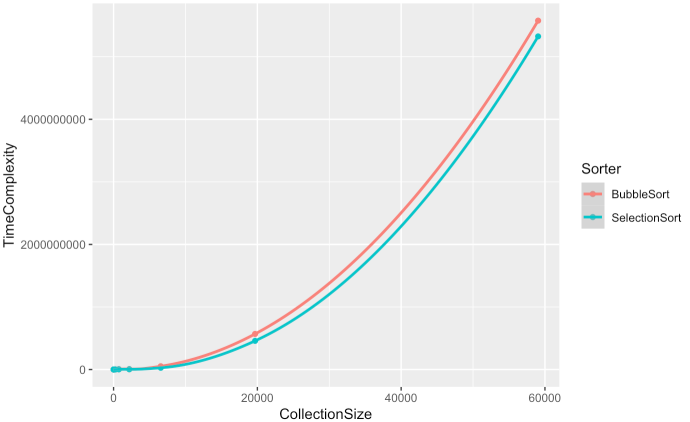
\includegraphics[width=0.7\linewidth]{FocusedViewOnBigTimeComplexity}
	\caption[Figure 3]{Focused view on the sub-group with higher time complexity}
	\label{fig:focusedviewonbigtimecomplexity}
\end{figure}
\newpage
Taking a focused look at the sub-group with higher time complexity, we can see that both of the sorters have a similar growth of Time Complexity, that leaves BubbleSort with slightly higher value of Complexity. The Growth here is similliar to a linear one and closer to the one that can be viewed on the Overall results view.
\section{Discussion}
- Small intro on the purpouse of the section here.
\subsection{Interpretation}
- Extended analysis on our graphs
- Deny or Approve our Hypothesis(Partially aprove it)
\subsection{Considerations}
- Limitations of the Machine used
- Limitations of the Emperical type of Analysis
\subsection{Evaluations}
- Simple Evaluation of our findings
\end{document}
	
	
\printbibliography[title=References]
R. Lafore. Data Structures and Algorithms in Java. SAMS
Publishing, Indianapolis, Indiana, USA, 2nd edition, 2002.

[2]Bunse, C., Hopfner, H., Mansour, E. and Roychoudhury, S., n.d. Exploring the Energy Consumption of Data Sorting Algorithms in Embedded and Mobile Environments. [online] citeseerx.ist.psu.edu. Available at: <https://citeseerx.ist.psu.edu/viewdoc/download?doi=10.1.1.543.8109&rep=rep1&type=pdf> [Accessed 14 December 2021].

[1]Sedgewick, R. & Wayne, K. (2011), Algorithms, 4th Edition. , Addison-Wesley .
\end{document}          
